\documentclass{article}

\usepackage{kern}

\begin{document}
    \subsection{Parameteroptimierung}
        \subsubsection*{Kapazitätsoptinierung}

            \begin{figure}
                \centering
                \begin{subfigure}[t]{0.45\textwidth}
                    \centering
                    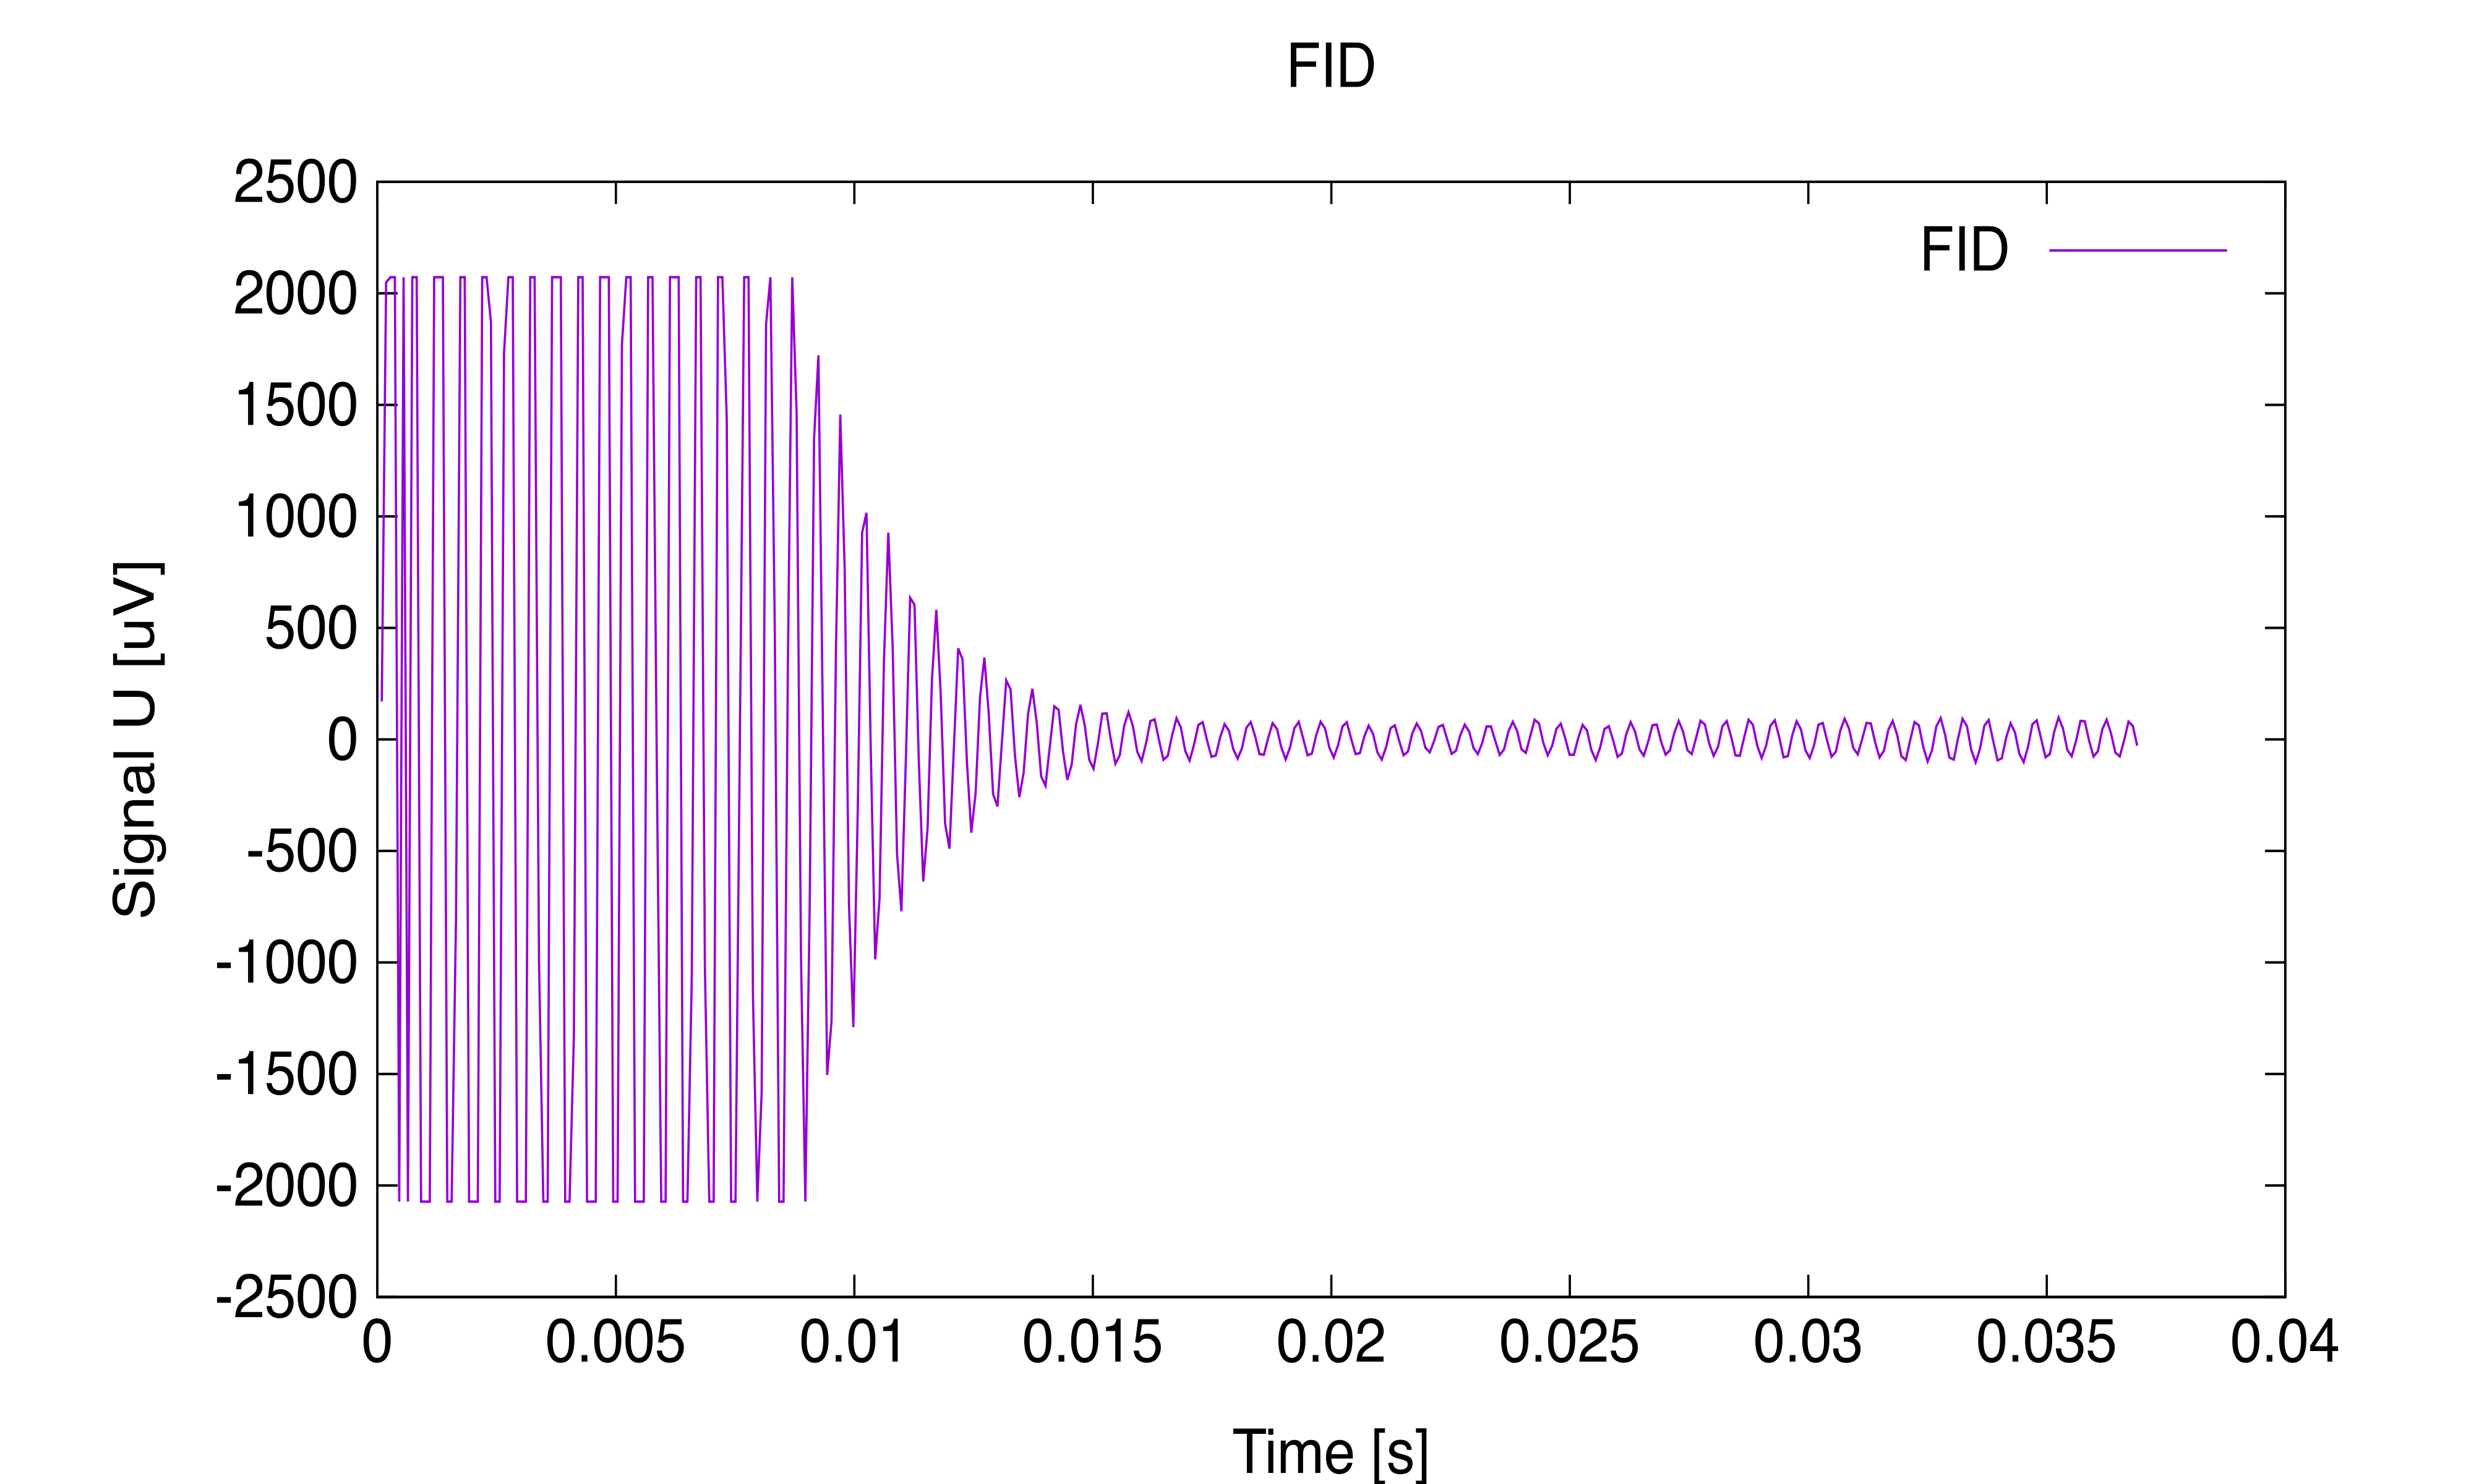
\includegraphics[width=6cm]{../Bilddateien/C_Opti_FID.png}
                    \caption{Messung der FID-Amplitude mit optimierter Kapazität.}
                \end{subfigure}
                \
                \begin{subfigure}[t]{0.45\textwidth}
                    \centering
                    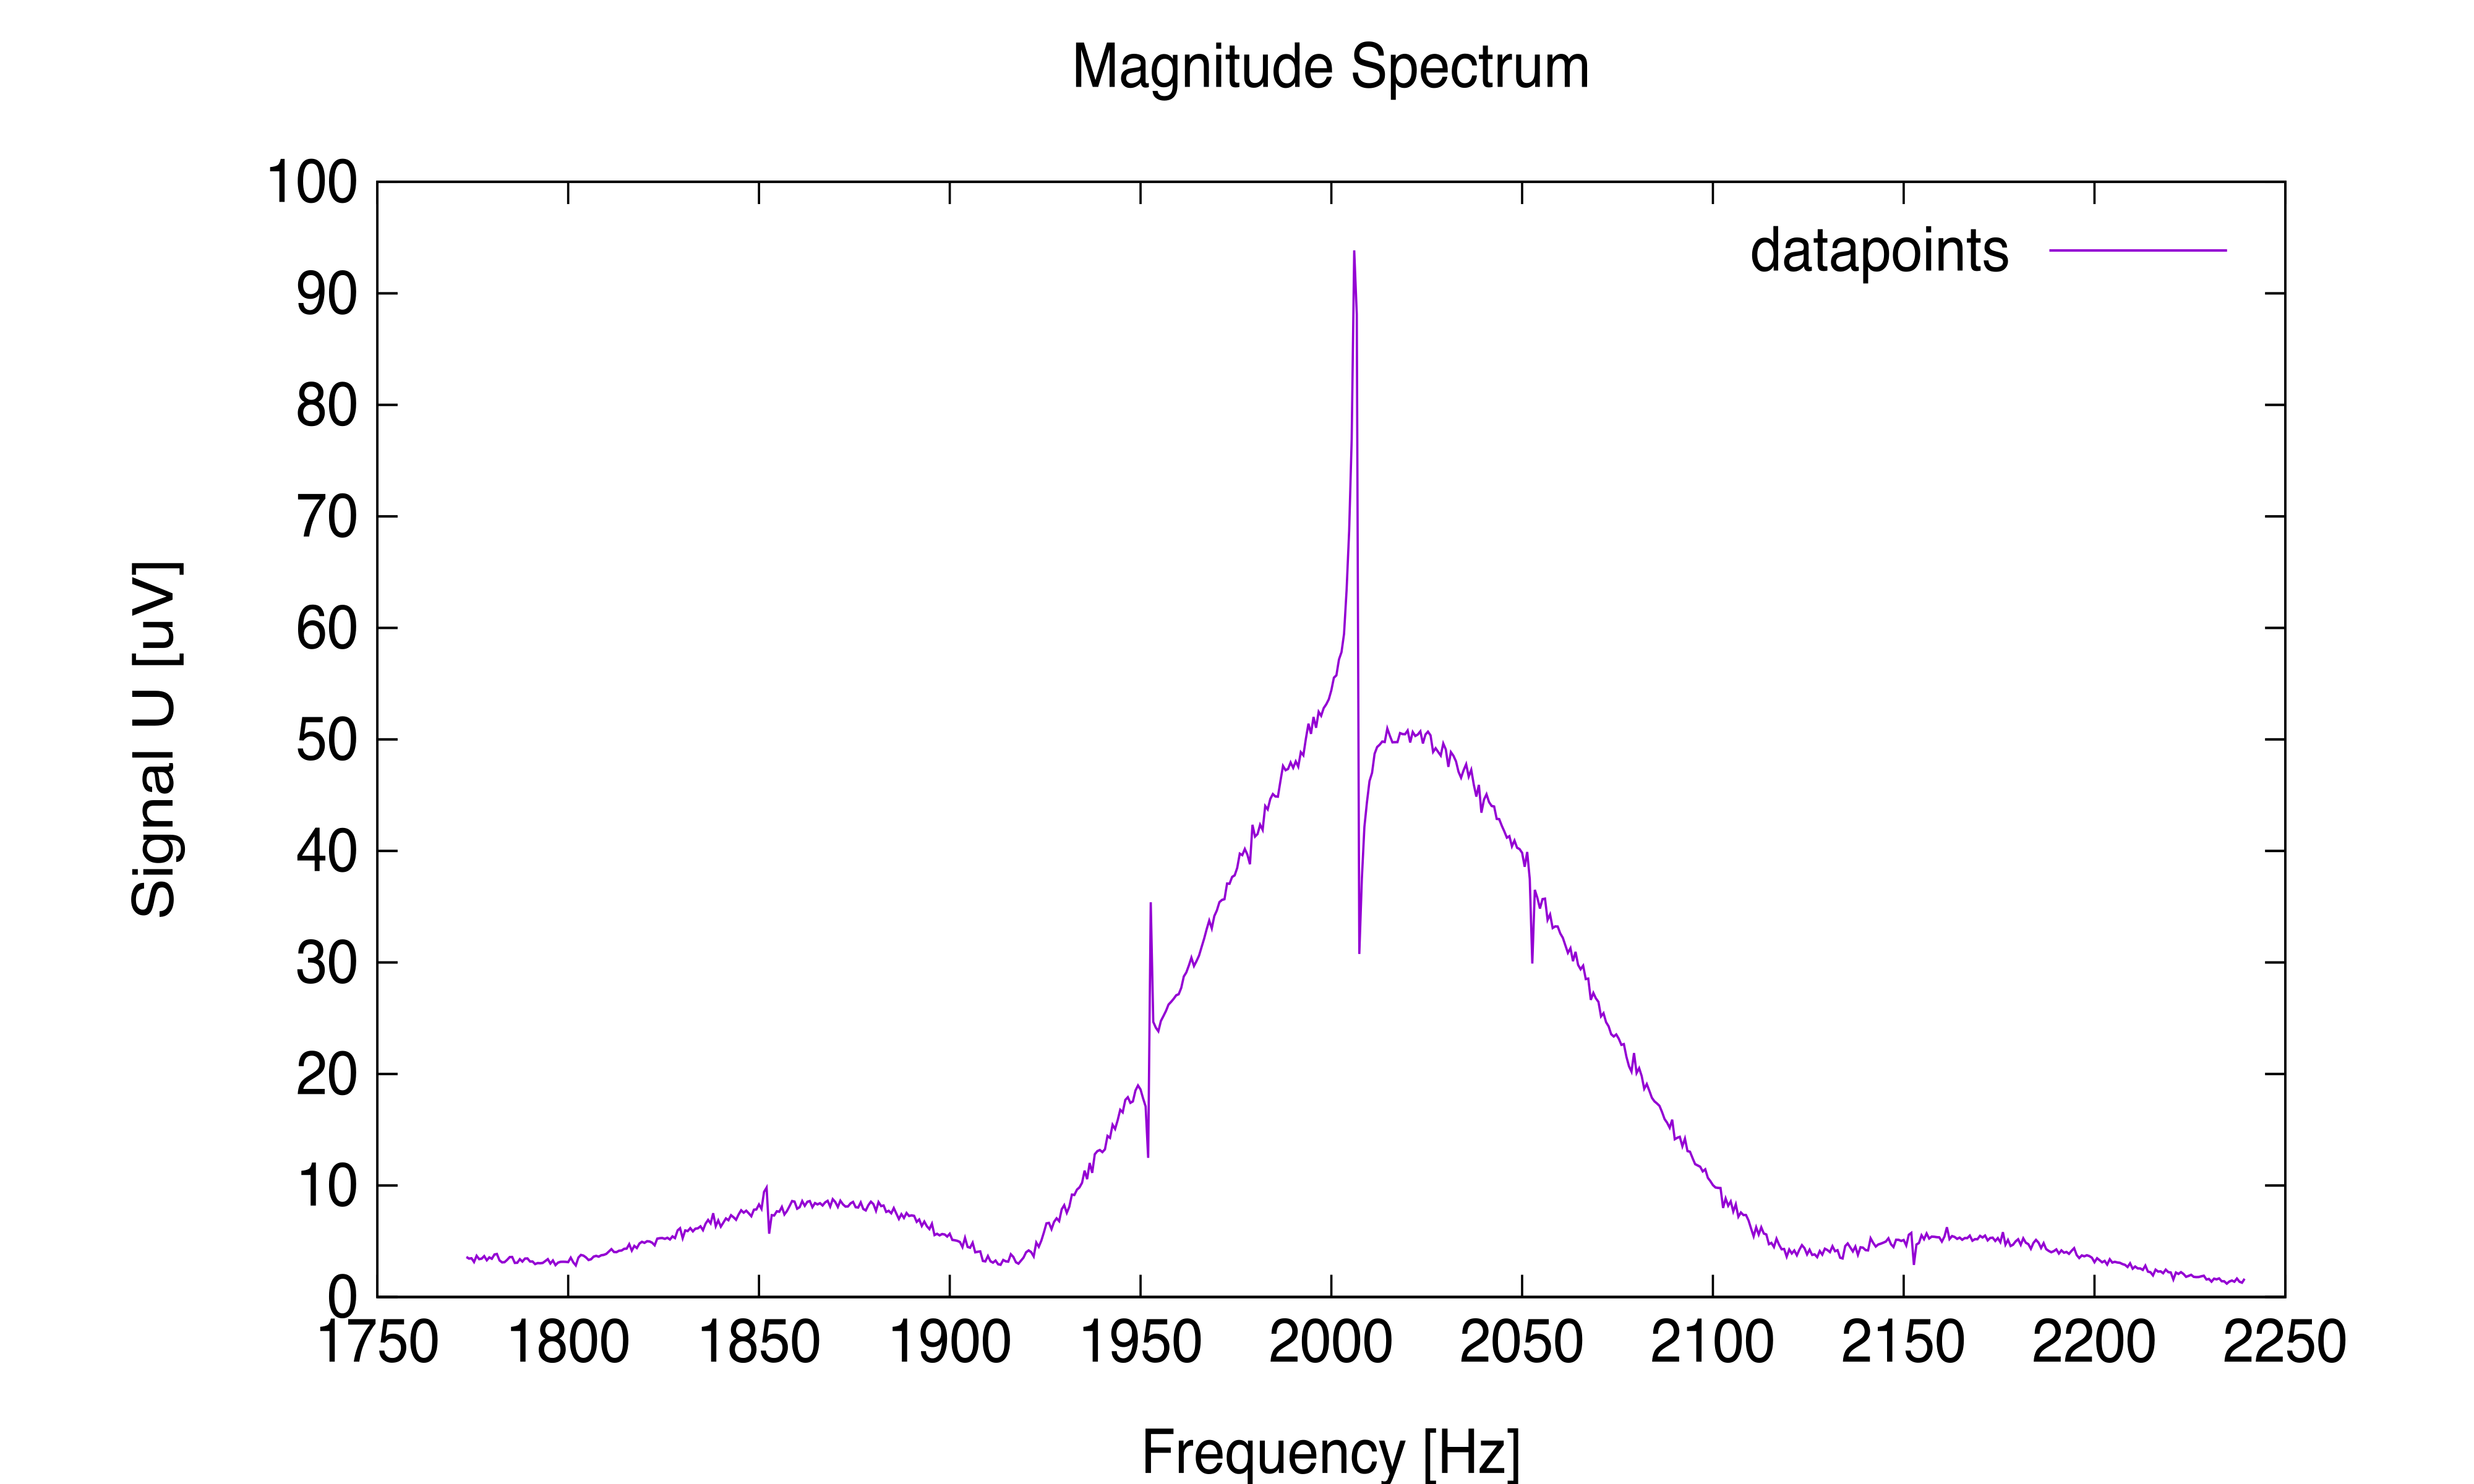
\includegraphics[width=6cm]{../Bilddateien/C_Opti_Spectrum.png}
                    \caption{Messung des Spektrums mit optimierter Kapazität.}
                \end{subfigure}
                \caption{Messung der FID-Amplitude und des Spektrums mit optimierter Kapazität.}
            \end{figure}
            Deutlich erkennbar ist die Larmor-Frequenz im Zentrum des Resonanzpeaks des LC-Schwingkreises. 

        \subsubsection*{Optimierung der $B_1$ Pulsdauer}

        \begin{figure}
            \centering
            \begin{subfigure}[t]{0.45\textwidth}
                \centering
                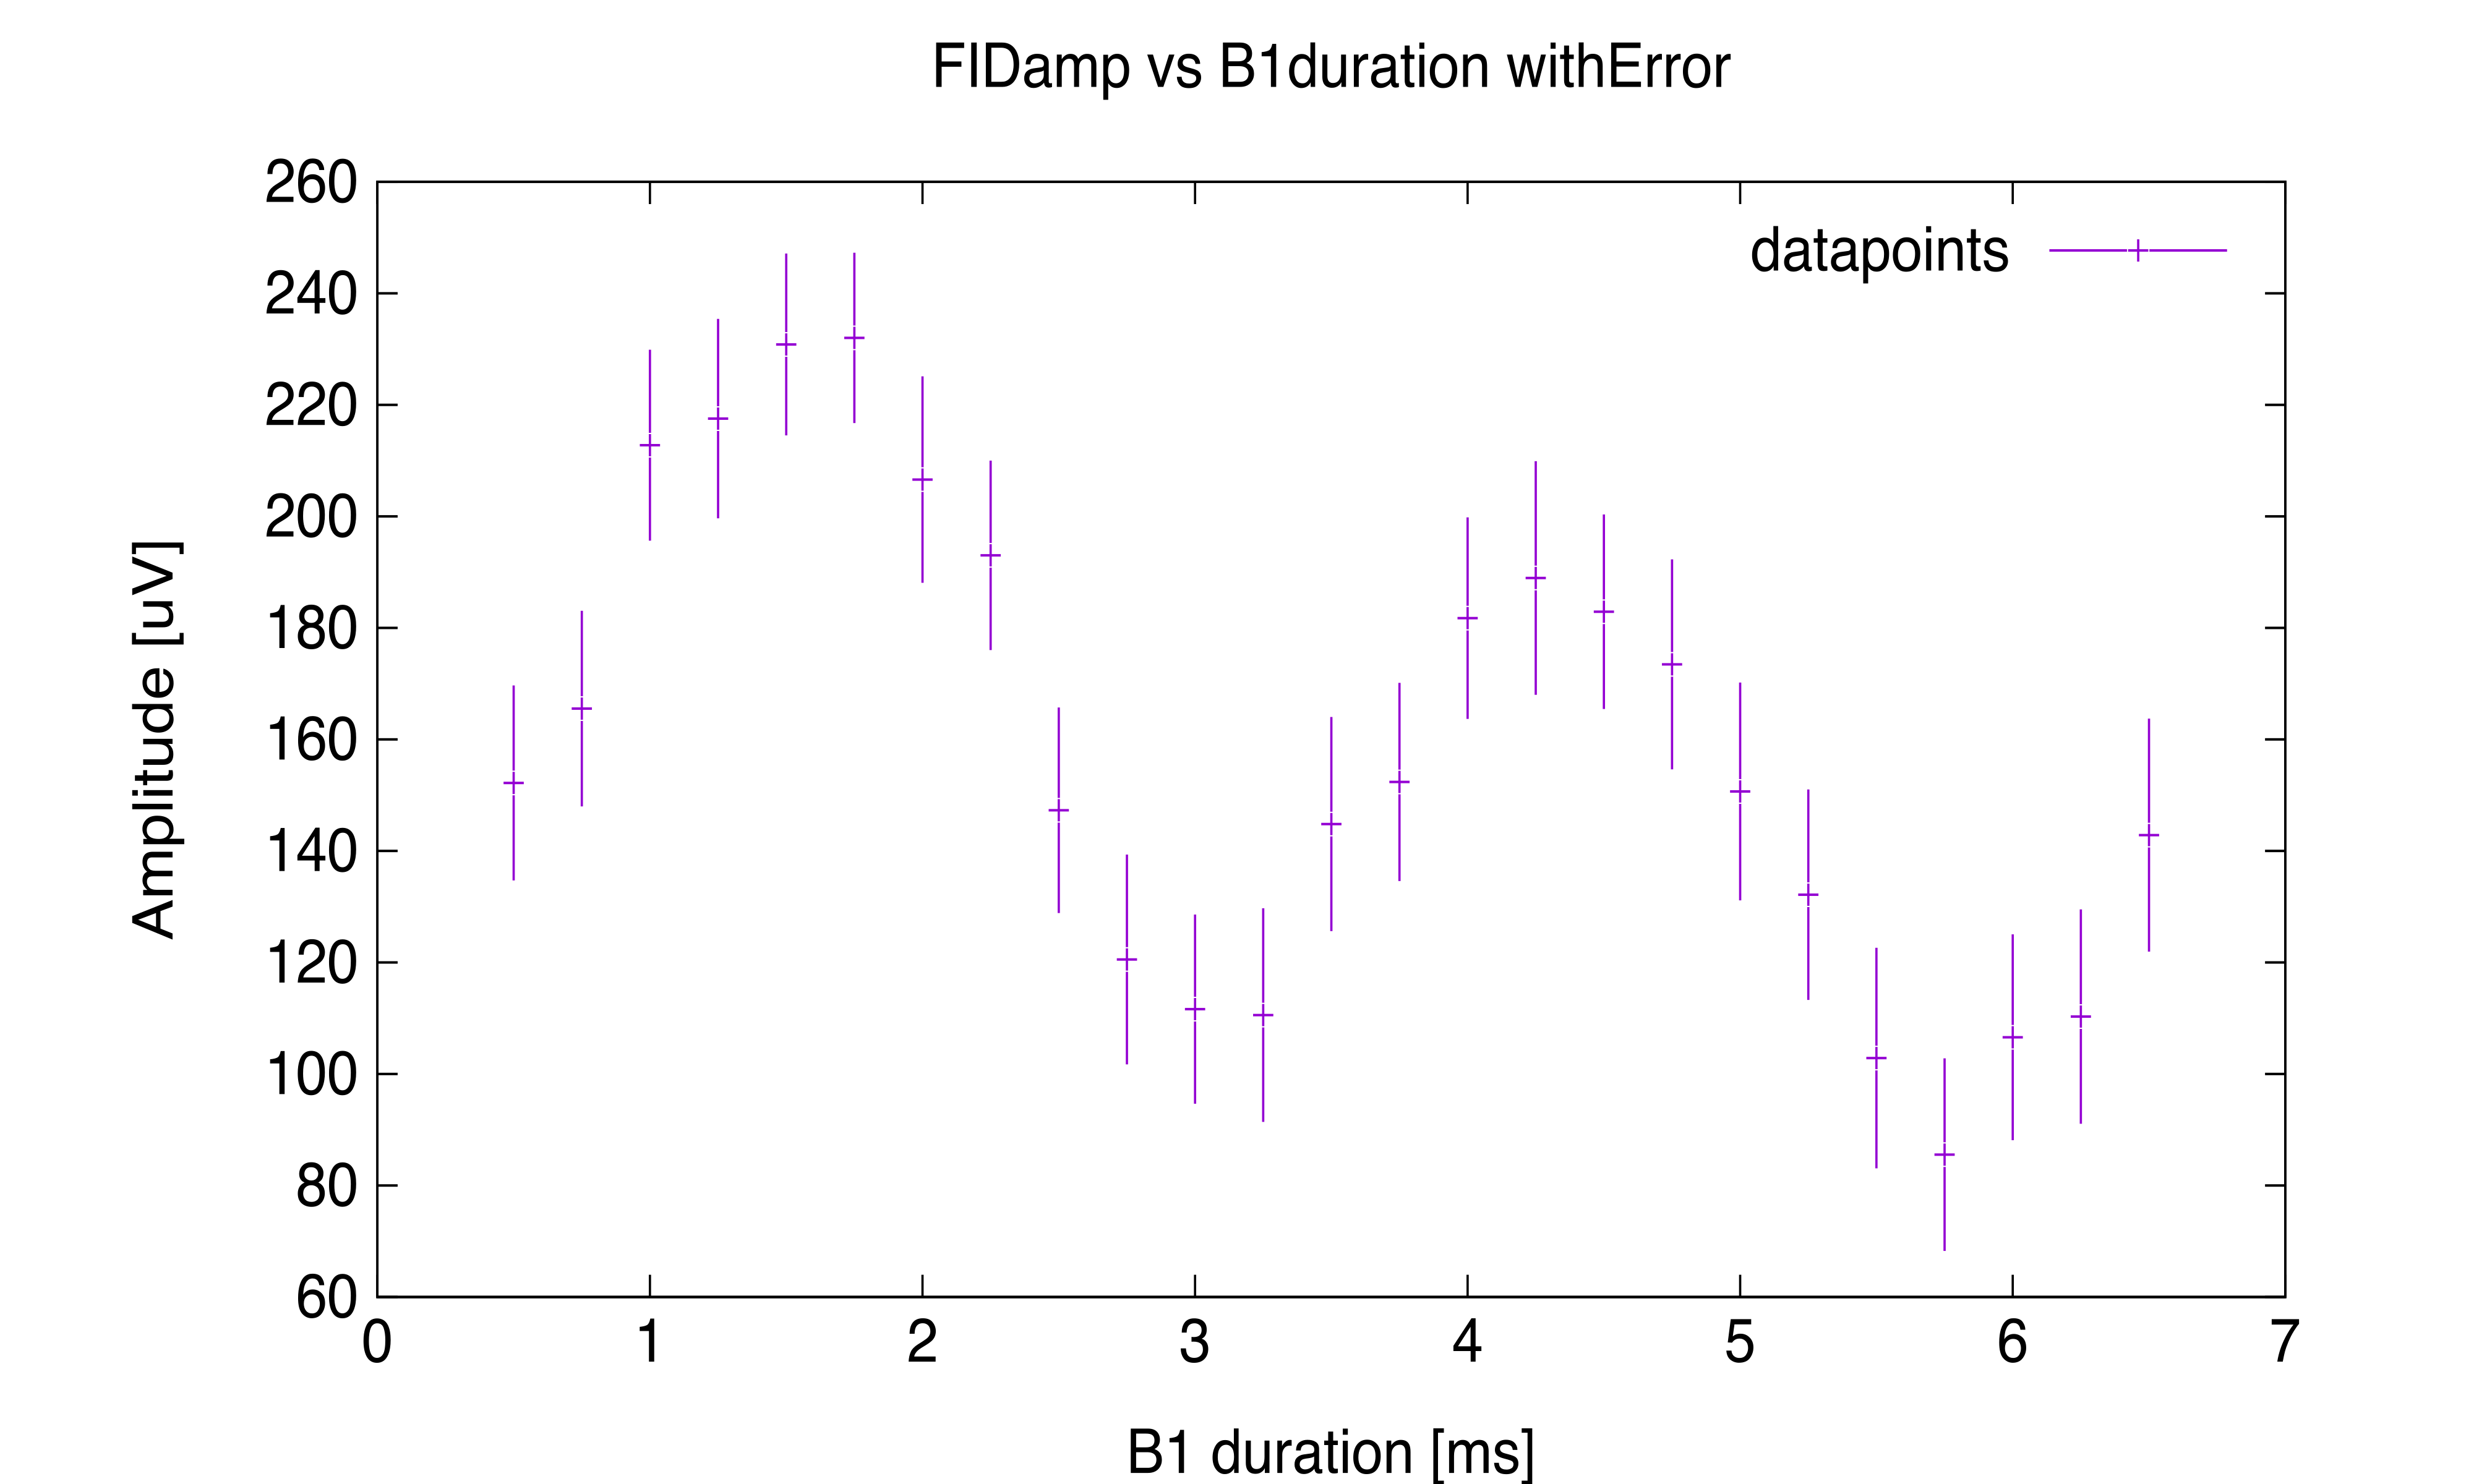
\includegraphics[width=6cm]{../Bilddateien/B1DurationFast_FIDamp_vs_B1duration_withError.png}
                \caption{Messung der FID-Amplitude mit Fehlerbalken in Abhängigkeit der B1-Dauer.}
                \label{fig:5:FastFIDampVsB1durationWithError}
            \end{subfigure}
            \
            \begin{subfigure}[t]{0.45\textwidth}
                \centering
                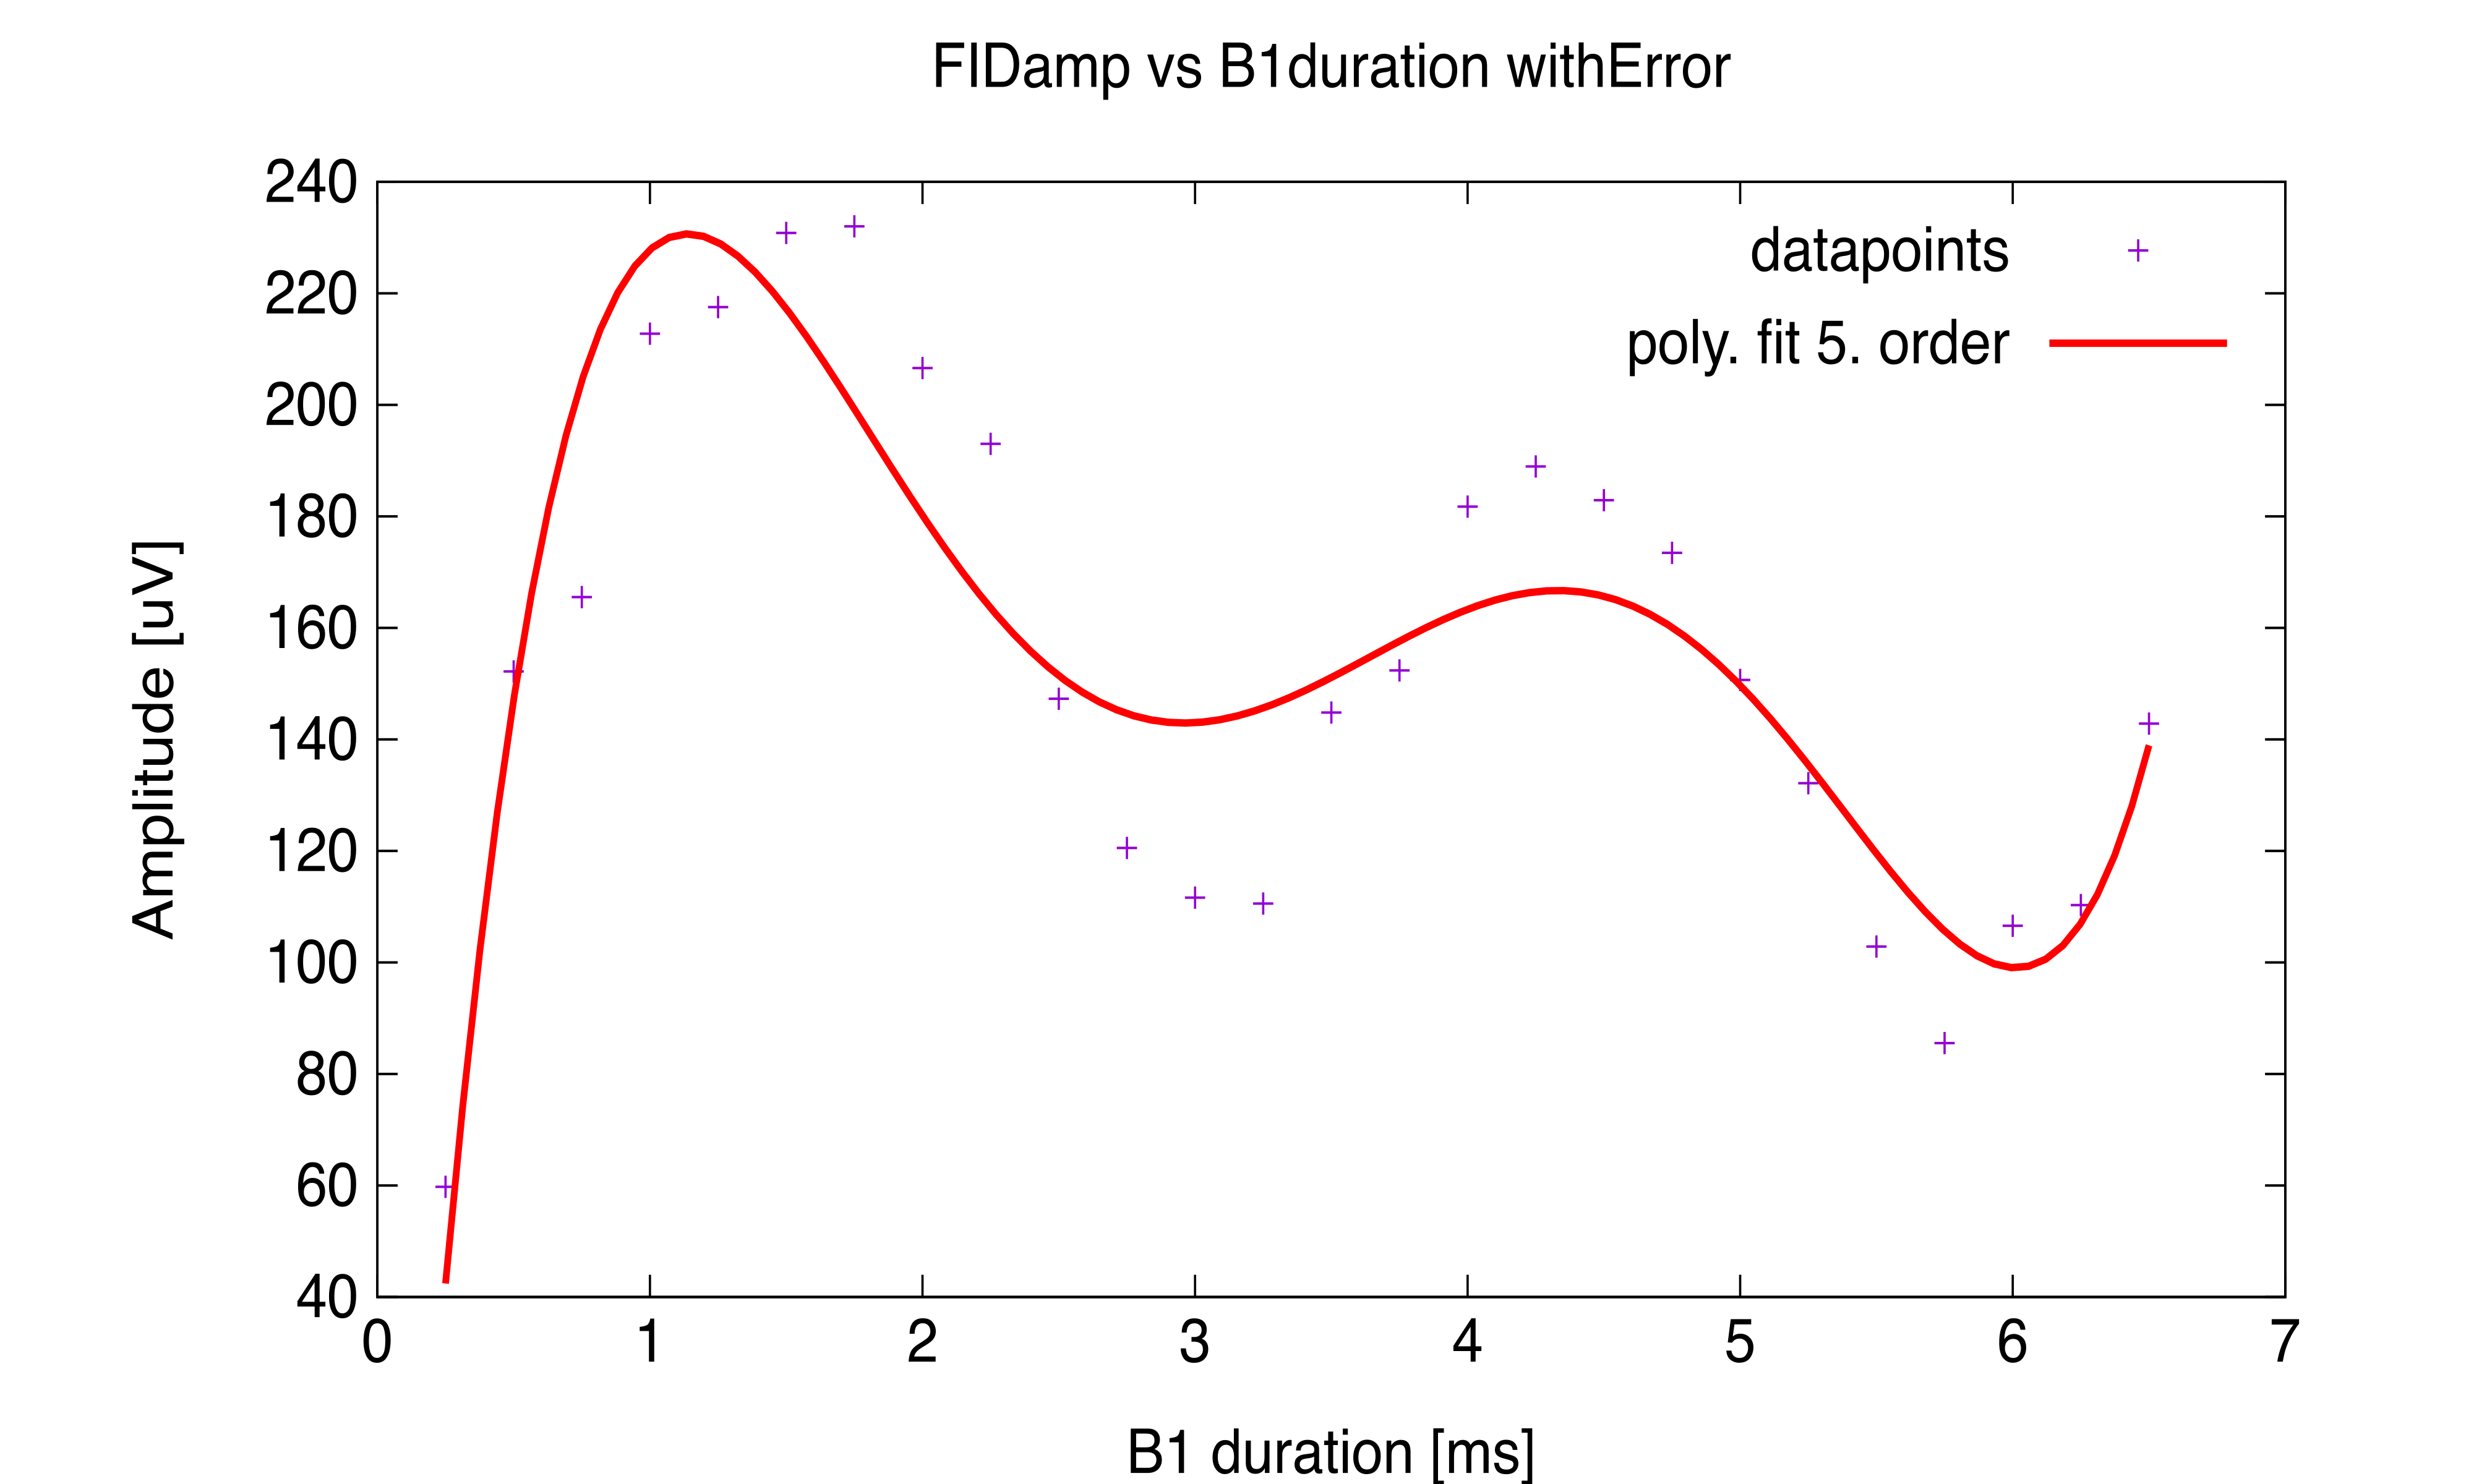
\includegraphics[width=6cm]{../Bilddateien/B1DurationFast_FIDamp_vs_B1duration_withError_poly.png}
                \caption{Messung der FID-Amplitude in Abhängigkeit der B1-Dauer mit polynomialer Kurvenanpassung fünfter Ordnung.}
                \label{fig:5:FastFIDampVsB1duration}
            \end{subfigure}
            \caption{Messung der FID-Amplitude in Abhängigkeit der B1-Dauer.}
        \end{figure}
\end{document}